\section{SimSite3D::Rectangular\-Solid Class Reference}
\label{classSimSite3D_1_1RectangularSolid}\index{SimSite3D::RectangularSolid@{SimSite3D::RectangularSolid}}
A rectangular bounding volume.  


{\tt \#include $<$Bounding\-Volume.H$>$}

Inheritance diagram for SimSite3D::Rectangular\-Solid::\begin{figure}[H]
\begin{center}
\leavevmode
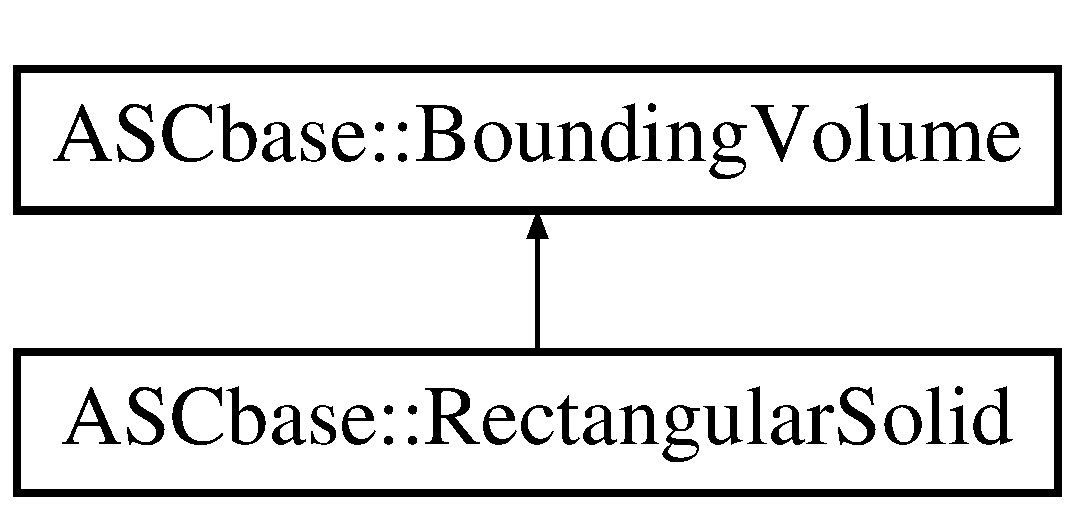
\includegraphics[height=2cm]{classSimSite3D_1_1RectangularSolid}
\end{center}
\end{figure}
\subsection*{Public Member Functions}
\begin{CompactItemize}
\item 
\textbf{Rectangular\-Solid} (const my\_\-float\_\-t $\ast$min\_\-corner\_\-in, const my\_\-float\_\-t $\ast$max\_\-corner\_\-in, const my\_\-float\_\-t grid\_\-spacing=0.0)\label{classSimSite3D_1_1RectangularSolid_6f27151311ea6c7c3036f033e55ce5bb}

\item 
\textbf{Rectangular\-Solid} (const \bf{Rectangular\-Solid} \&src)\label{classSimSite3D_1_1RectangularSolid_52a293bc179ad6858cf4c7f06937a224}

\item 
virtual bool \bf{contains} (const my\_\-float\_\-t $\ast$point) const \label{classSimSite3D_1_1RectangularSolid_a9e2c2a9ec3c034f3bba17219a7116c2}

\begin{CompactList}\small\item\em Is the given point inside the bounding volume? \item\end{CompactList}\item 
virtual bool \textbf{BIND\_\-vol\_\-contains} (const my\_\-float\_\-t $\ast$p) const \label{classSimSite3D_1_1RectangularSolid_3d17933ceada4081756d2e3f4a8bf6d2}

\item 
virtual bool \textbf{RAD\_\-vol\_\-contains} (const my\_\-float\_\-t $\ast$p) const \label{classSimSite3D_1_1RectangularSolid_888d6eb616e675241d0a3d11fb330a4f}

\item 
virtual size\_\-t \bf{discretize} (const my\_\-float\_\-t spacing, my\_\-float\_\-t $\ast$$\ast$grid\_\-pts)\label{classSimSite3D_1_1RectangularSolid_39443291990068ad369c9edfc75a4e76}

\begin{CompactList}\small\item\em discretize the volume using the spacing for grid spacing. \item\end{CompactList}\item 
virtual std::string \textbf{xml\_\-str} ()\label{classSimSite3D_1_1RectangularSolid_a8acf31a229ca25907a0d6cb85da4ec3}

\end{CompactItemize}
\subsection*{Private Attributes}
\begin{CompactItemize}
\item 
my\_\-float\_\-t \textbf{min\_\-corner} [3]\label{classSimSite3D_1_1RectangularSolid_a57a2744d2006581f35568bd2e43ea58}

\item 
my\_\-float\_\-t \textbf{max\_\-corner} [3]\label{classSimSite3D_1_1RectangularSolid_6d297afcc473c3cc2336c3017e7f638a}

\item 
my\_\-float\_\-t \textbf{BIND\_\-min\_\-corner} [3]\label{classSimSite3D_1_1RectangularSolid_fdbc647071b0beff1c695f5919eecf14}

\item 
my\_\-float\_\-t \textbf{BIND\_\-max\_\-corner} [3]\label{classSimSite3D_1_1RectangularSolid_bd9eb2d180cd46f6325a483d809c17f5}

\item 
my\_\-float\_\-t \textbf{RAD\_\-min\_\-corner} [3]\label{classSimSite3D_1_1RectangularSolid_f06af8b6554856ea2fb19d943c1a5b3b}

\item 
my\_\-float\_\-t \textbf{RAD\_\-max\_\-corner} [3]\label{classSimSite3D_1_1RectangularSolid_463d6a3ed40fa149db9cdccd456cd075}

\end{CompactItemize}


\subsection{Detailed Description}
A rectangular bounding volume. 



The documentation for this class was generated from the following files:\begin{CompactItemize}
\item 
Bounding\-Volume.H\item 
Bounding\-Volume.C\end{CompactItemize}
